\documentclass{jcgt}

\setciteauthor{Collin Boots, Dalton Banks}
\setcitetitle{GPU-Accelerated Conversion of RGBD Images to Textured Triangle Meshes}

% Mark submissions with the date of submission using the following line:
%\submitted{\today}

% Once an article is accepted accepted, switch to the following line and comment the preceding one. The editor will supply the argument values.
%\accepted{July 4, 2013}{July 4, 2013}{July 4, 2013}{Editor Name}{2}{1}{1}{1}{2013}
%\seturl{http://jcgt.org/published/0002/02/01/}




%%%%%%%%%%%%%%%%%%%%%%%%%%%%%%%%%%%%%%%%%%%%%%%%%%%%


\begin{document}

\title{GPU-Accelerated Conversion of RGBD Images to Textured Triangle Meshes}

\author
       {Collin Boots\\University of Pennsylvania
        \and Dalton Banks\\University of Pennsylvania
       }

% Optional teaser image
\teaser{
  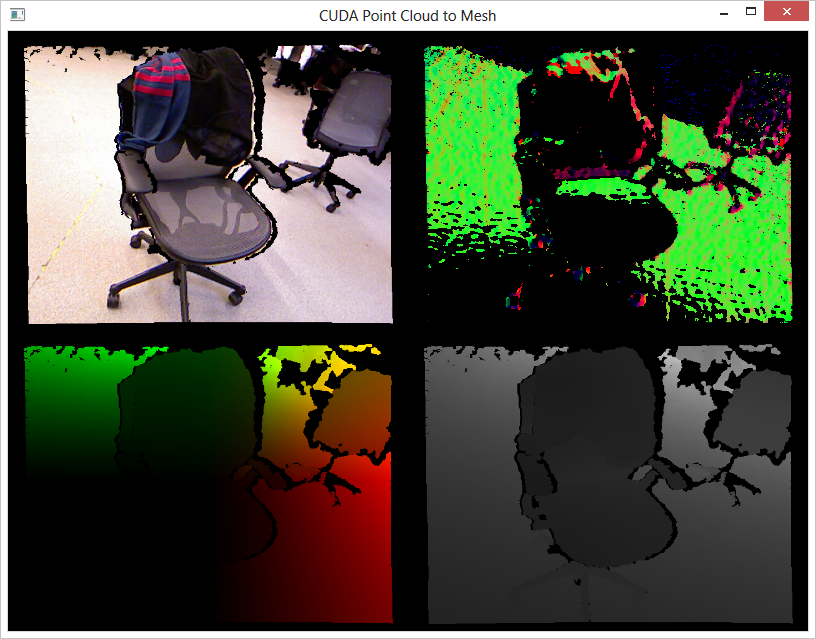
\includegraphics[width=3in]{../../screenshots/ChairPointCloudNormals.PNG}
  
  \label{fig:teaser}
  \caption{Depth data (placeholder)}
}


\maketitle
%\thispagestyle{firstpagestyle}

\begin{abstract}
\small
Mesh reconstruction from low-cost RGBD cameras, as opposed to simple point cloud storage, holds many possibilities, such as ease of object recognition and greatly reduced memory requirements. A modular framework was developed for extracting and synchronizing RGB and depth data from an RGBD camera, performing CUDA-based data processing on a GPU, and rendering the transformed data with OpenGL via CUDA-OpenGL interop on the GPU. In particular, data was gathered from the Microsoft Kinect using OpenNI, CUDA kernels were used to perform neighborhood-based estimation of point normals and dense surface mesh reconstruction in camera-space, and a variety of GLSL shaders were implemented to visualize the processed data. Further work will extend the framework to perform image registration of successive RBGD frames for reconstruction from camera movement, and will perform adaptive mesh resampling in order to further decrease memory usage.
\end{abstract}


%-------------------------------------------------------------------------
\section{Introduction}
\label{sec:introduction}
Previous work has demonstrated the diverse capabilities of RGBD cameras, from generating highly accurate 3D surface models \cite{KinectFusion} to reliably estimating 3D pose \cite{Endres,Taguchi}. However, many algorithms attempt to store the generated environment as a RGB 3D point cloud, which is not easily adaptable to dynamic environments, requires enormous quantities of memory to store large environments, and provides no intuition to higher perception processes about distinct objects beyond a volumetric approximation. Other approaches have been able to store and merge the surface data more efficiently, but still regard the environment as a unified whole rather than discrete objects. By instead extracting meaningful geometry from the RGBD data in the form of triangle meshes, many advantages can be realized:

\begin{enumerate}
\item High storage efficiency
\item Natural low level object segmentation
\item Easy to manipulate, modify, and render in real time
\item Efficient and easy to process intuition of geometry that higher cognitive functions can use for object recognition and manipulation tasks.
\item Straightforward tradeoff between simplicity and accuracy with mesh resolution
\end{enumerate}

\section{Code Overview}
\subsection{Image processing pipeline}
The overall image processing pipeline is shown in Figure~\ref{fig:imgProcPipeline}. First, an RGB frame and a depth frame are pulled from the Kinect and shipped to the GPU for processing. A world-space point cloud is then generated from the RGBD data, and a neighborhood-based estimate of the point normals is then extracted for later processing. Finally, the point cloud is triangulated and the generated mesh is passed to OpenGL where a variety of rendering options are implemented.

\begin{figure}[htb]
  \centering
   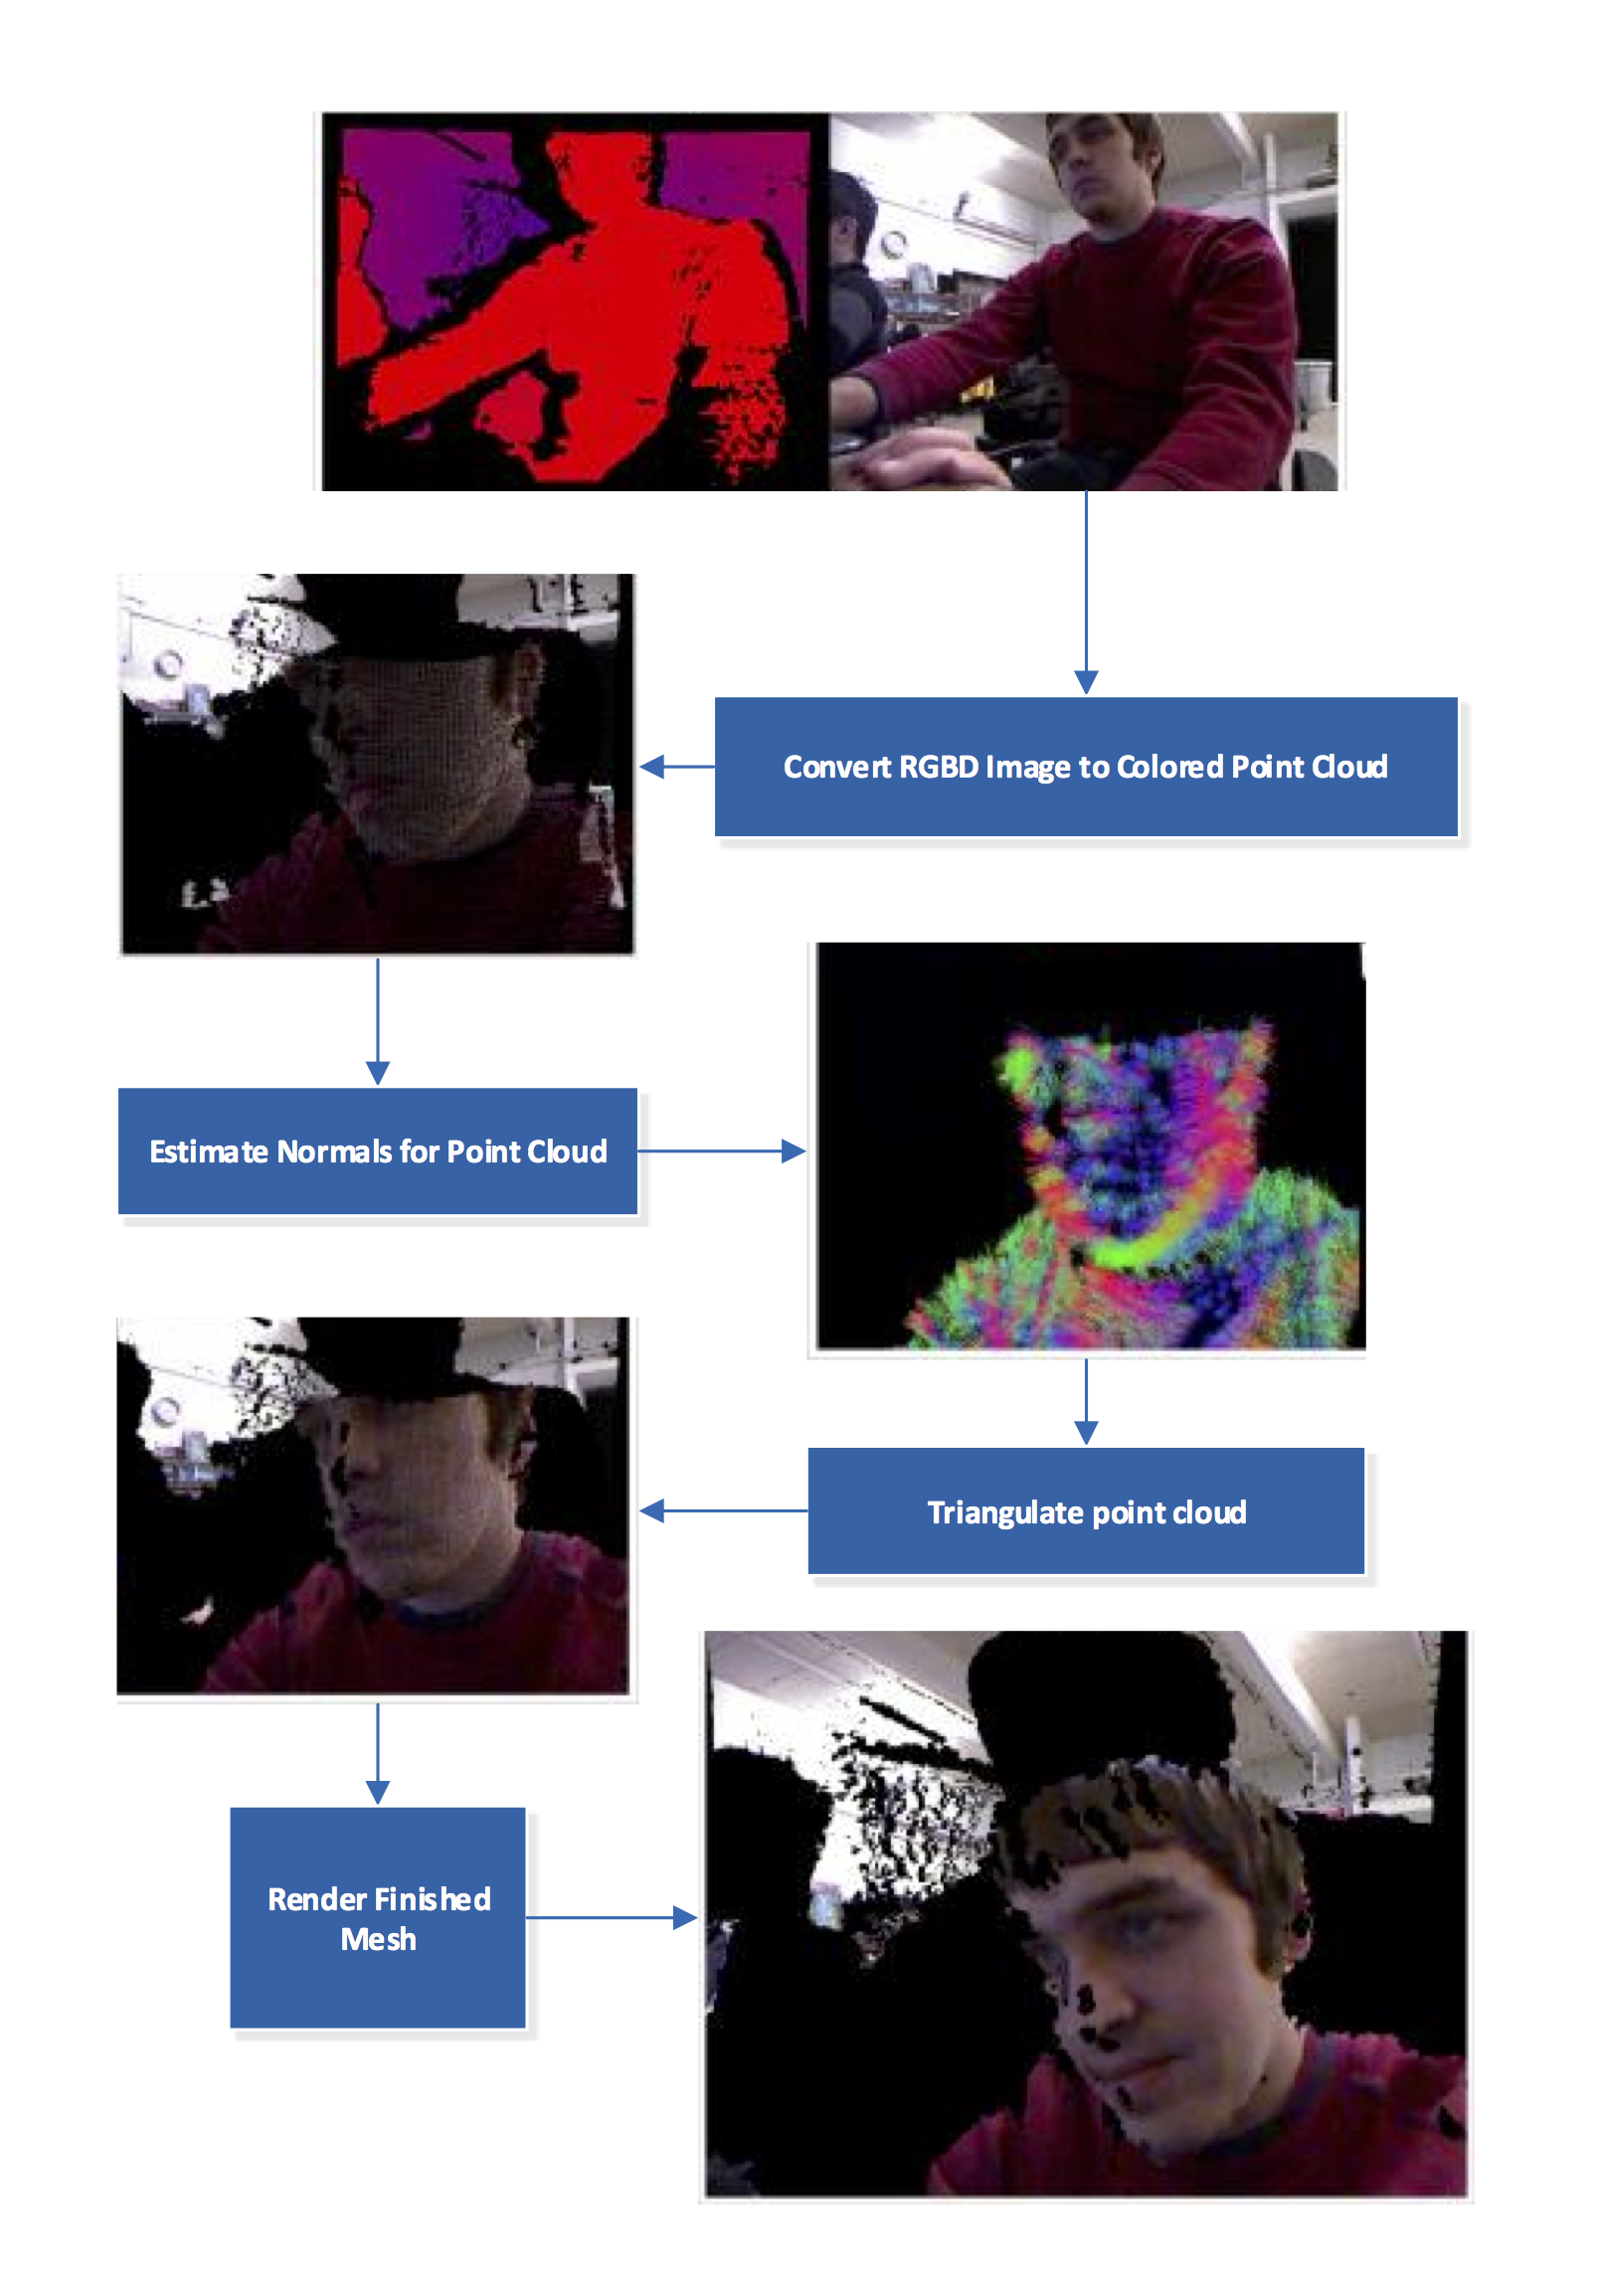
\includegraphics[width=0.8\textwidth]{../../diagrams/ImageProcessingPipeline.png}
   \caption{\label{fig:imgProcPipeline}
        Image Processing Pipeline}
\end{figure}

The underlying architecture is very modular, and can be easily extended to handle input RGBD streams other than the Kinect (as demonstrated in the implementation of log streams). A generic RGBD frame format is used, allowing computation and visualization to be performed without regard to how the data was obtained.

A more detailed view of the program flow is shown in Figure~\ref{fig:progFlow}. Note that after the RGB and depth frames are synchronized and shipped to the GPU, all computation and rendering is performed on the GPU, enhancing performance and allowing the CPU to be free for other tasks. The ComputeNormalsFast kernel supplants an earlier iteration, ComputeNormals, which was written for estimation quality at the cost of a significant performance penalty.

\begin{figure}[htb]
  \centering
   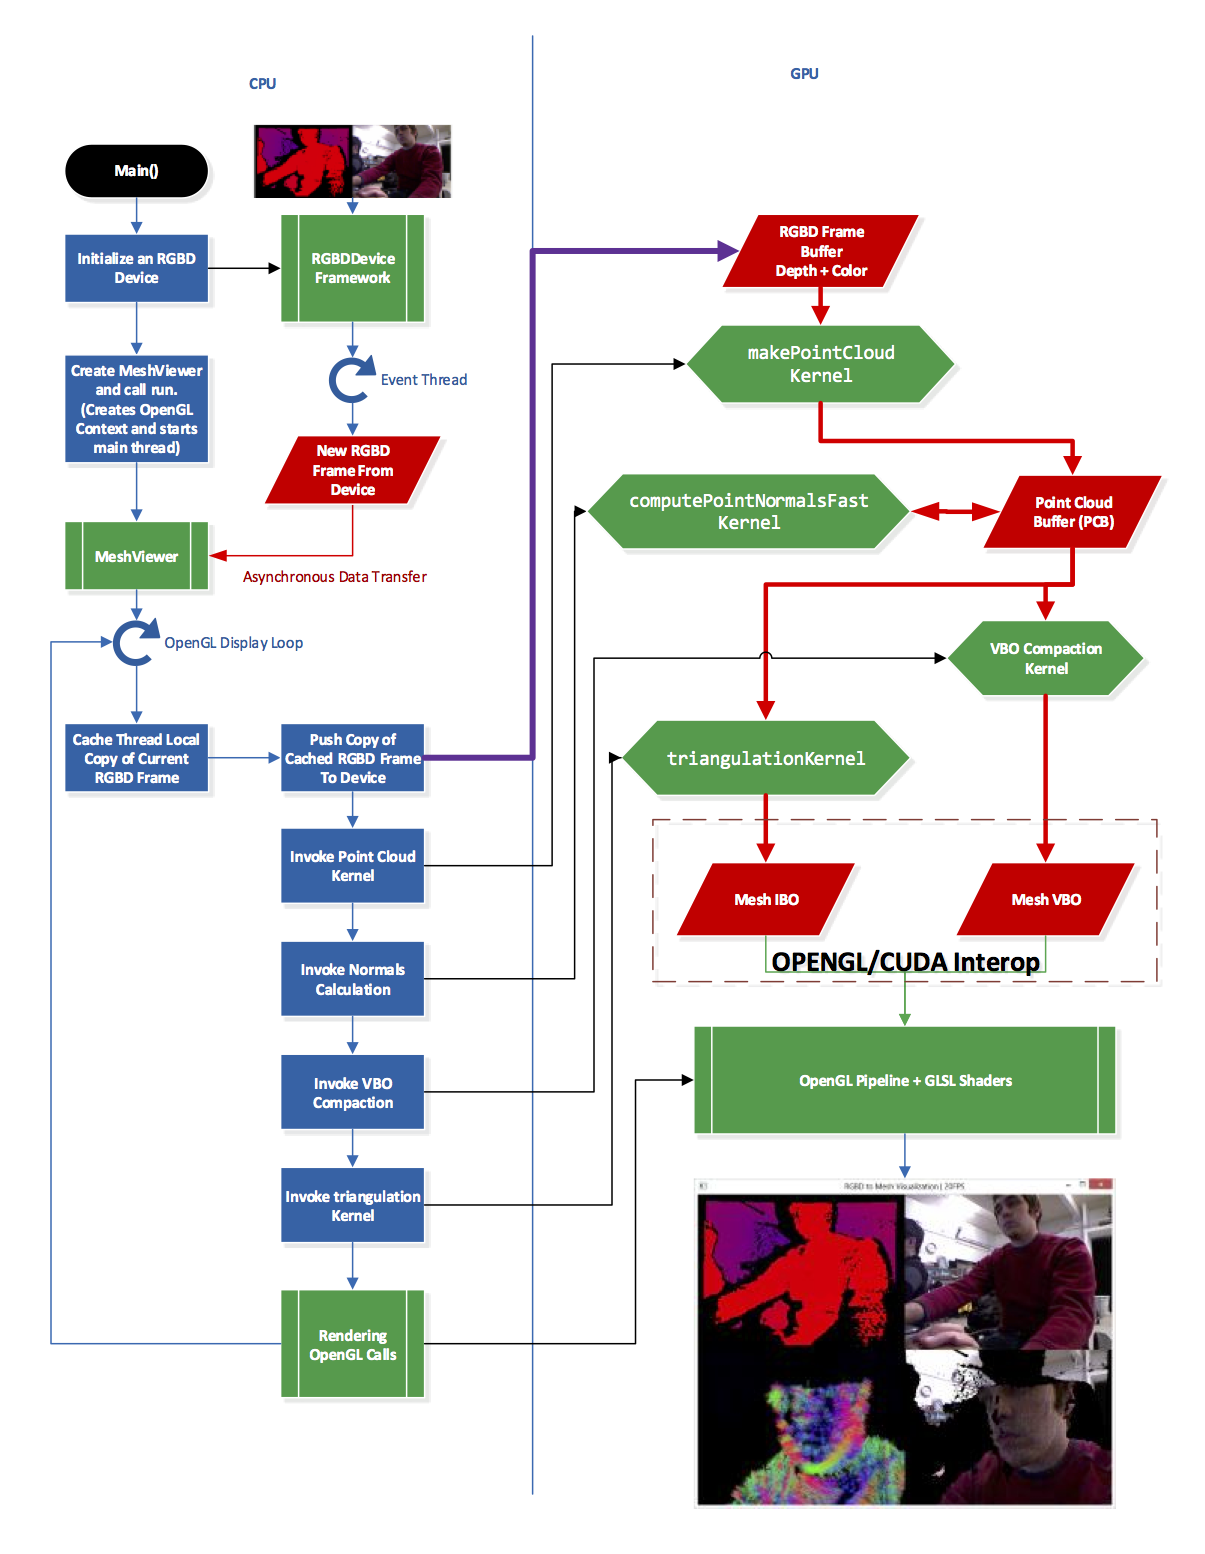
\includegraphics[width=0.8\textwidth]{../../diagrams/ProgramFlow.png}
   \caption{\label{fig:imgProcPipeline}
        Overall Program Flow}
\end{figure}

Finally, Figure~\ref{fig:GLPipeline} shows a more detailed view of the OpenGL rendering pipeline. The rendering pipeline is also written in a very modular manner, allowing both for rapid code modification to experiment with different visualazation techniques, as well as hooks (note the black diamonds) for keypresses to completely change the render output on-the-fly.

\begin{figure}[htb]
  \centering
   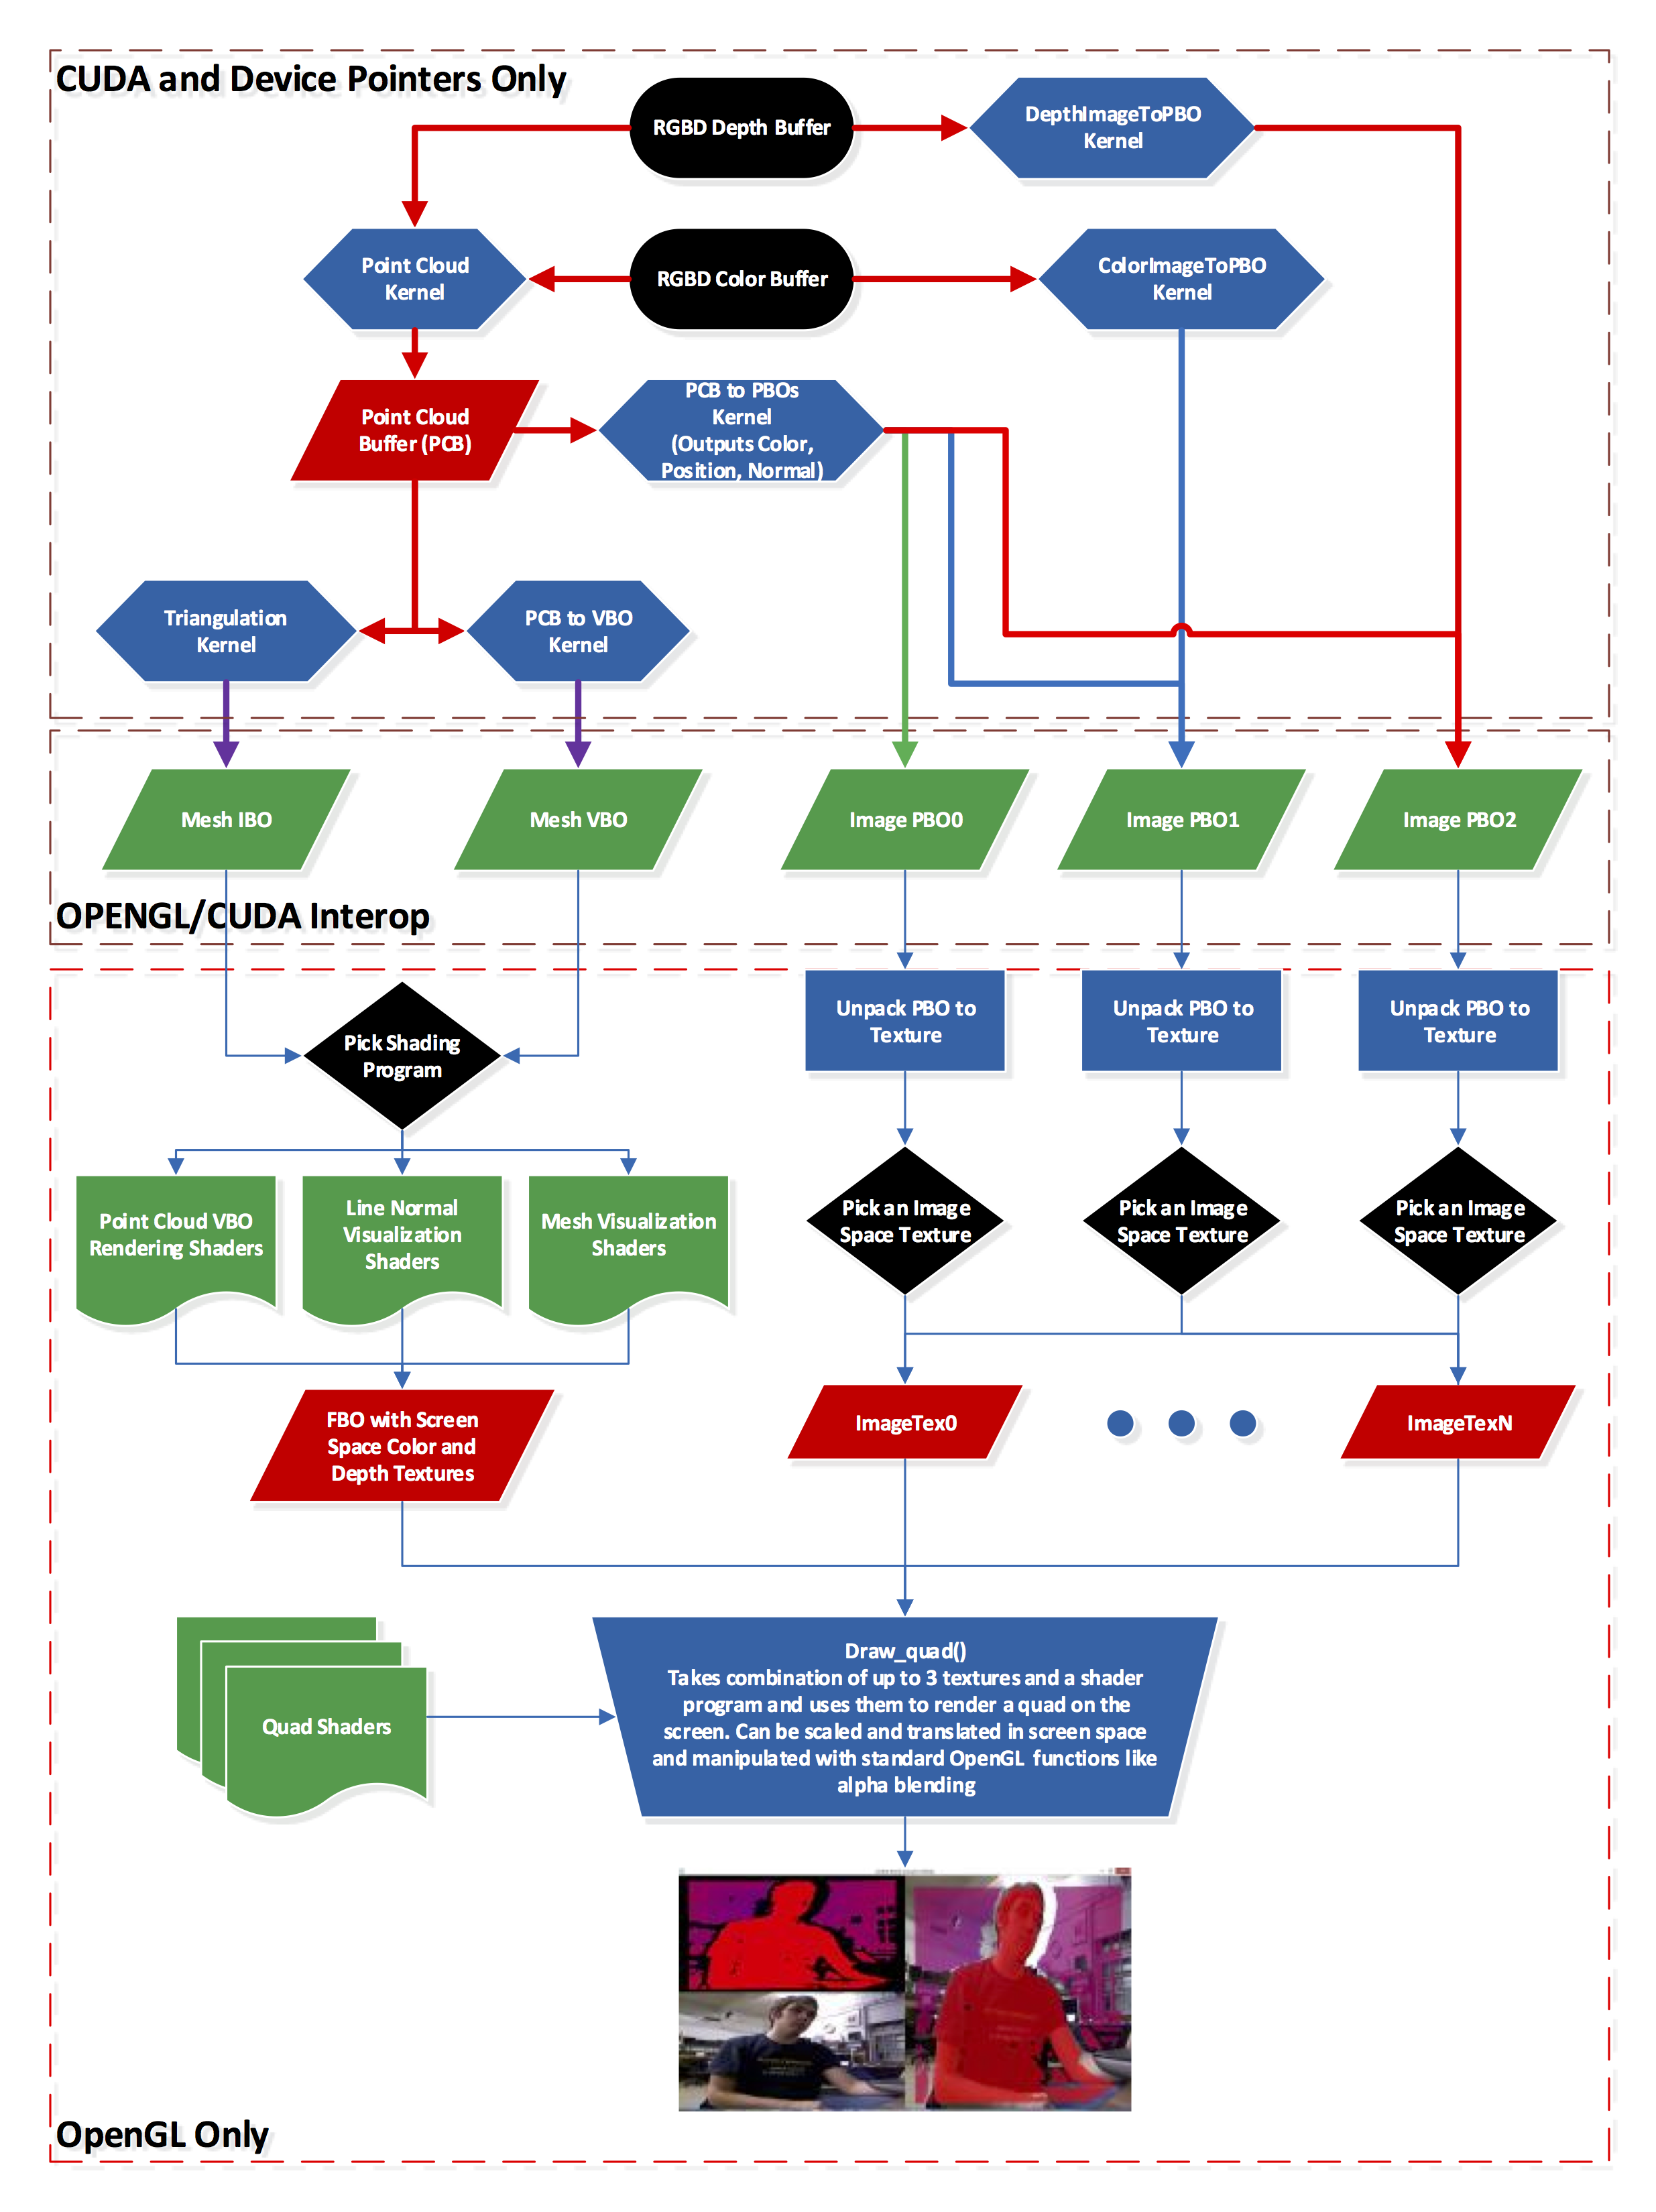
\includegraphics[width=0.8\textwidth]{../../diagrams/OpenGLPipeline.png}
   \caption{\label{fig:GLPipeline}
        OpenGL Pipeline}
\end{figure}

\section{Performance Analysis}

Our point normals kernel was implemented as follows. A window radius is first specified as an algorithm parameter. For each point, we loop through its neighboring points in screen space in the square window specified by the radius, and pair it with a screen-space orthogonal point at the same radius. If both points are within a specified radius from the center point in world space, we take the cross product to compute the normal, which is then flipped if pointing away from the camera. If sufficiently many valid normals are found, we average them to produce the final normal estimate, otherwise we discard the point.

To improve the runtime of the point normals kernel, we reimplemented the algorithm using shared memory. In the shared memory implementation, all points in given thread block are first loaded into shared memory, along with the points lying within the specified neighborhood radius of the edges of the thread block, and the distance and cross product calculations are then performed using shared memory access. The results of the shared memory optimization on kernel runtime are shown for a range of window radii using a thread block size of 8x8.

\begin{figure}[htb]
  \centering
   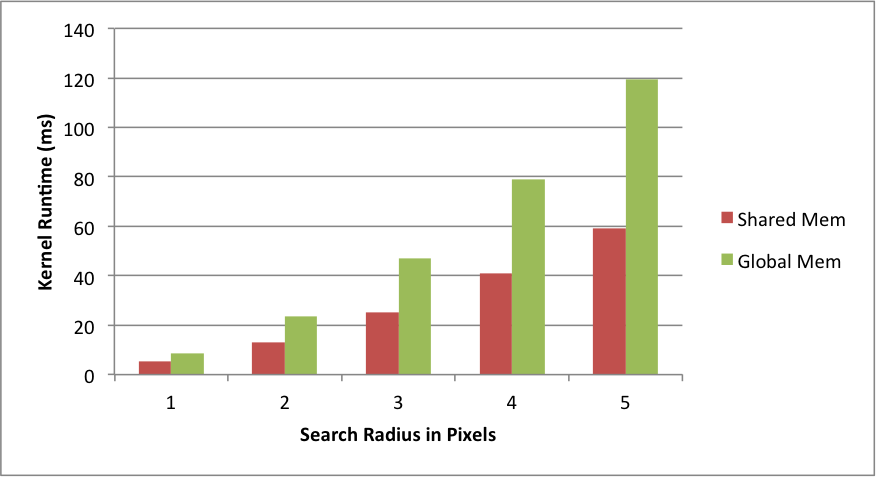
\includegraphics[width=0.8\textwidth]{../../performance/SharedVsGlobalRuntime.png}
   \caption{\label{fig:GLPipeline}
    Global vs. shared memory access: kernel runtime}
\end{figure}

\begin{figure}[htb]
  \centering
   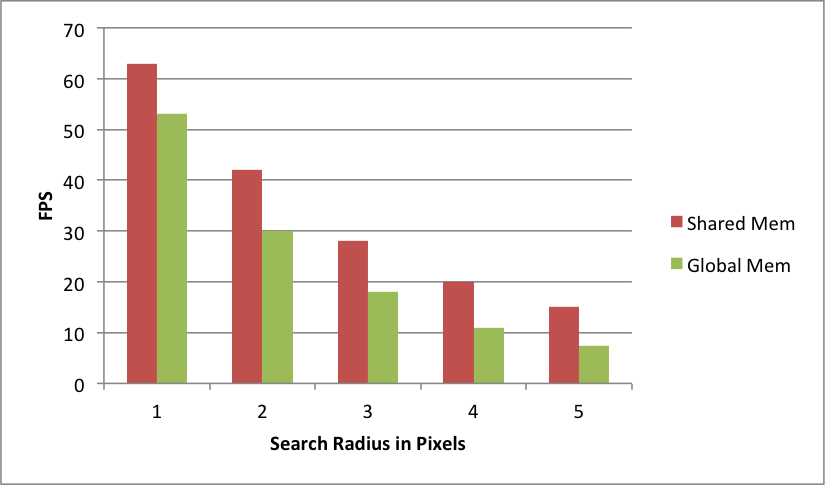
\includegraphics[width=0.8\textwidth]{../../performance/SharedVsGlobalFPS.png}
   \caption{\label{fig:GLPipeline}
    Global vs. shared memory access: frame rate}
\end{figure}

As demonstrated, the shared memory optimization reduced the kernel runtime by approximately a factor of 2. The impact on the overall FPS was less dramatic, though still pronounced, due to the time spent in the rendering pipeline. All testing for this project was conducted on an Intel Core i5-2450M CPU, 2.5GHz 6GB (Windows 8, 64-bit OS) and an NVIDIA GeForce GT 525M GPU.


%\subsection*{Acknowledgements}
%This project makes use of the following 3rd party libraries: \href{http://www.boost.org/}{Boost}, \href{http://nvlabs.github.io/cub/}{CUB}, \href{https://code.google.com/p/thrust/}{Thrust}, \href{https://code.google.com/p/lz4/}{LZ4}, \href{http://rapidxml.sourceforge.net/}{RapidXML}. The project was done for Patrick Cozzi's CIS 565 GPU Programming class at the University of Pennsylvania, Fall 2013.
%
\small
\bibliographystyle{acmsiggraph}
\bibliography{report}

%\section*{Author Contact Information}
%
%\hspace{-2mm}\begin{tabular}{p{0.5\textwidth}p{0.5\textwidth}}
%Collin Boots \newline
%University of Pennsylvania\newline
%\href{mailto:cboots@seas.upenn.edu}{cboots@seas.upenn.edu}
%&
%
%Dalton Banks \newline
%University of Pennsylvania\newline
%\href{mailto:dbanks@seas.upenn.edu}{dbanks@seas.upenn.edu} \newline
%\href{http://graphica.edu/~rtrace}{http://graphica.edu/\textasciitilde rtrace}
%
%\end{tabular}


%\afterdoc

\end{document}
